%! TEX root = diss.tex
\documentclass[../diss.tex]{subfiles}

\appendix

\chapter{Definitions and proofs}%
\label{cha:Further definitions}

% {{{

\section{Abstract algebra}%
\label{sec:Abstract algebra}

A group $(G, \bullet)$ consists of a set $G$ and an operator $\bullet$ that takes
two elements of $G$ and gives a new element in $G$. A group also:
\begin{itemize}
    \item is closed under $\bullet$
    \item the operator is associative
    \item There is a neutral element $e \in G$
    \item Each element $a \in G$ has an inverse $b$ such that $a \bullet b=e=b \bullet a$
\end{itemize}

An \textit{abelian} group is a group that also has the property of commutativity,
that is $a \bullet b = b \bullet a$ for all $a,b \in G$.

A \textit{monoid} meets all the properties of a group, except that there is
no requirements for there to be an inverse element for each $a \in G$.

A \textit{ring} $(R, \oplus, \otimes)$ consists of a set $R$ and operators
$\oplus, \otimes : R \times R \rightarrow R$ with the properties:
\begin{itemize}
    \item $(R, \oplus)$ meets the requirements of an abelian group
    \item $(R, \otimes)$ meets the requirements of a monoid
    \item $a \times (b \oplus c)$ for elements in $R$ follow the distributive law
\end{itemize}

In a \textit{semiring}, we meet all the requirements of a ring, except there is
no requirement for the addition operator $\oplus$ to have inverses for all elements.

A \textit{tropical semiring} is the class of the \textit{min} semiring $(\mathbb{R} \cup \{\infty\}, \oplus, \otimes)$ where
\begin{itemize}
    \item $\oplus = \min$
    \item $\otimes = +$
\end{itemize}
and the \textit{max} semiring $(\mathbb{R} \cup \{-\infty\}, \oplus, \otimes)$ where
\begin{itemize}
    \item $\oplus = \min$
    \item $\otimes = +$
\end{itemize}

\section{Proof of correct addition in generalised FoxOtto}%
\label{sec:Proof of correct addition in generalised FoxOtto}

In \cref{sec:APSP via repeated matrix-squaring}, I claimed
\begin{quote}
    ``\textit{it can be shown that on line 17 [in \cref{alg:foxOtto}], we are computing
    $A[i',k] + B[k,j']$ with $i',j'$ and $k$ as defined on lines 14--16}.''
\end{quote}

Consider the computation of $A'[i_2,m]+B'[m,j_2]$ for some arbitrary valid values
for $n,p,i,j,i_2,j_2$ and $m$. 
Because of the input padding, we will have $n'=n/p$ (without rounding).
We want to show that $(\dagger): A'[i_2,m]=A[i', k]$
and $(\ddagger): B'[m,j_2]=B[k,j']$.

\textbf{Proof of $(\dagger)$:}

We first show the first index matches:
By definition, $i'=i\cdot n' + i_2$, so $A[i',k]=A[i\cdot n/p + i_2,k]=A'[i_2,k]$
by how we distribute the input.

On line 9, we receive from broadcast the submatrix of $A$ along the $j$th
column, where $j=(i+l) \mod p$. We also have $k=(n' \cdot (i+l)+m) \mod n$. 
This gives 
\begin{align}
    A'[i_2,m] &=A[i',((i+l) \mod p)\cdot n'+m], \textrm{ by translating from index of submatrix} \\
    & = A[i', (i+l)\cdot n' \mod (p\cdot n')+m] \\
    & = A[i', (i+l)\cdot n' \mod n+m] \\
    & = A[i', ((i+l)\cdot n'+m) \mod n], \textrm{ because } m < n \\
    & = A[i', k], \textrm{ QED}
\end{align}

\textbf{Proof of $(\ddagger)$:}

The proof of this is similar because the shift-pattern moves submatrices
$B'$ such that after $l$ iterations, the submatrix that originally belonged to
\ac{PE} $(i,j)$ will be at location $(i,j=(i+l)\mod p)$, which is the same
congruence as above.

% }}}

\chapter{Java unit tests and various scripts used}

% Unit tests {{{
\section{Unit tests}%
\label{sec:Unit tests}

The layout of the \texttt{.java} files that were part of the unit-testing is
found in \cref{fig:test-repo-overview}. The result of the unit tests is shown
in \cref{fig:unit-test-full}.

\begin{figure}[h]
\begin{center}
    \begin{adjustbox}{valign=t}
    \begin{forest}
        dirtree,
        [test/java/
            [APSPSolver/
                [MatSquareTest.java]
            ]
            [graphReader/
                [GraphCompressorTest.java]
            ]
            [matrixMultiplication/
                [BroadcastMatrixMultiplicationTest.java]
                [FoxOttoTest.java]
                [GeneralisedFoxOttoTest.java]
            ]
            [memoryModel/
                [CommunicationManagerTest.java]
            ]
            [timingAnalysis/
                [testWorkers/
                    [TestWorker1.java]
                    [TestWorker2.java]
                ]
                TimedCommunicationManagerTest.java
            ]
            [util/
                [MatrixTest.java]
            ]
            [work/
                [ManagerTest.java]
                [WorkerManagerExceptionTest.java]
                [WorkerTest.java]
            ]
        ]
    \end{forest}
\end{adjustbox}
\end{center}
\caption{The repository layout of the \texttt{test/java/} folder. Also see the associated result of the unit tests in \cref{fig:unit-test-full}.}
\label{fig:test-repo-overview}
\end{figure}


% }}}

% word count{{{

\section{Word count}%
\label{sec:Word count}

To manage the dissertation, I used the \texttt{subfiles} \LaTeX-package, so each
chapter is written in a separate \texttt{.tex} file.
To count the words, I concatenate the 5 chapters and use {\TeX}count%
\footnote{\url{https://ctan.org/pkg/texcount}}.
I used the following script to do this:
\begin{verbatim}
echo "$(head -n 4 diss.tex)
    $(tail -n +3 -q sections/*.tex)
    $(tail diss.tex -n +5 -q)" | \
    texcount - $@ -sub=chapter | \
    grep -P "Introduction|Preparation|Implementation|Evaluation|Conclusions" | \
    grep -oP "\d+[+]\d+[+]\d+" | \
    bc | \
    awk '{s+=$1} END {print s}'
\end{verbatim}
% }}}

% Final line count {{{
\section{Final line count}%
\label{sec:Final line count}

I counted the \texttt{main/java/} lines with:

\begin{verbatim}
find ParallelAPSP/src/main/java/ -name '*.java' | xargs wc -l
\end{verbatim}

and the lines in \texttt{test/java/} with:

\begin{verbatim}
find ParallelAPSP/src/test/java/ -name '*.java' | xargs wc -l
\end{verbatim}

To count the lines of Python code, I ran:

\begin{verbatim}
find scripts/ -name '*.py' | xargs wc -l
\end{verbatim}

and subtracted 53 from the total count (see \cref{sec:evaluation}).

% }}}


% random graphs{{{
\section{\texttt{random-graphs.py}}%
\label{sec:ttsdasdasd}

The \texttt{random-graphs.py} Python script was used to generate the input graphs
used in evaluation in \cref{fig:main-eval-plot}. I ran the following to generate
the inputs:

\begin{verbatim}
    create_and_save_graphs(calGraph, [10,20,30,40,50,60,70,80,90,100, \
        150,200,250,300,350,400,450,500,550,600,650,700], \
        "cal-compressed-random-graphs")
\end{verbatim}

% }}}

% graph extractor {{{

\section{\texttt{graph-extractor.py}}%
\label{sec:extract}

This script can extract subsections of the real-world graph datasets presented
by \citeauthor{graph-dataset} \cite{graph-dataset}. In \cref{fig:appendix-ol-small}, we see an example of this usage. This was used to generate the \texttt{OL-but-smaller.cedge} test dataset with 430 vertices, which was used as input to the unit
tests \texttt{graphCompressorCorrectlySolvesAPSPOnLargeGraphs()} and
\texttt{generalisedAPSPAlgorithmGivesCorrectResultOnLargeGraph}. These tests
checked that all paths between pairs $(i,j) \in V^2$ were computed and
reconstructed correctly.

\begin{figure}[h!]
    \begin{center}
        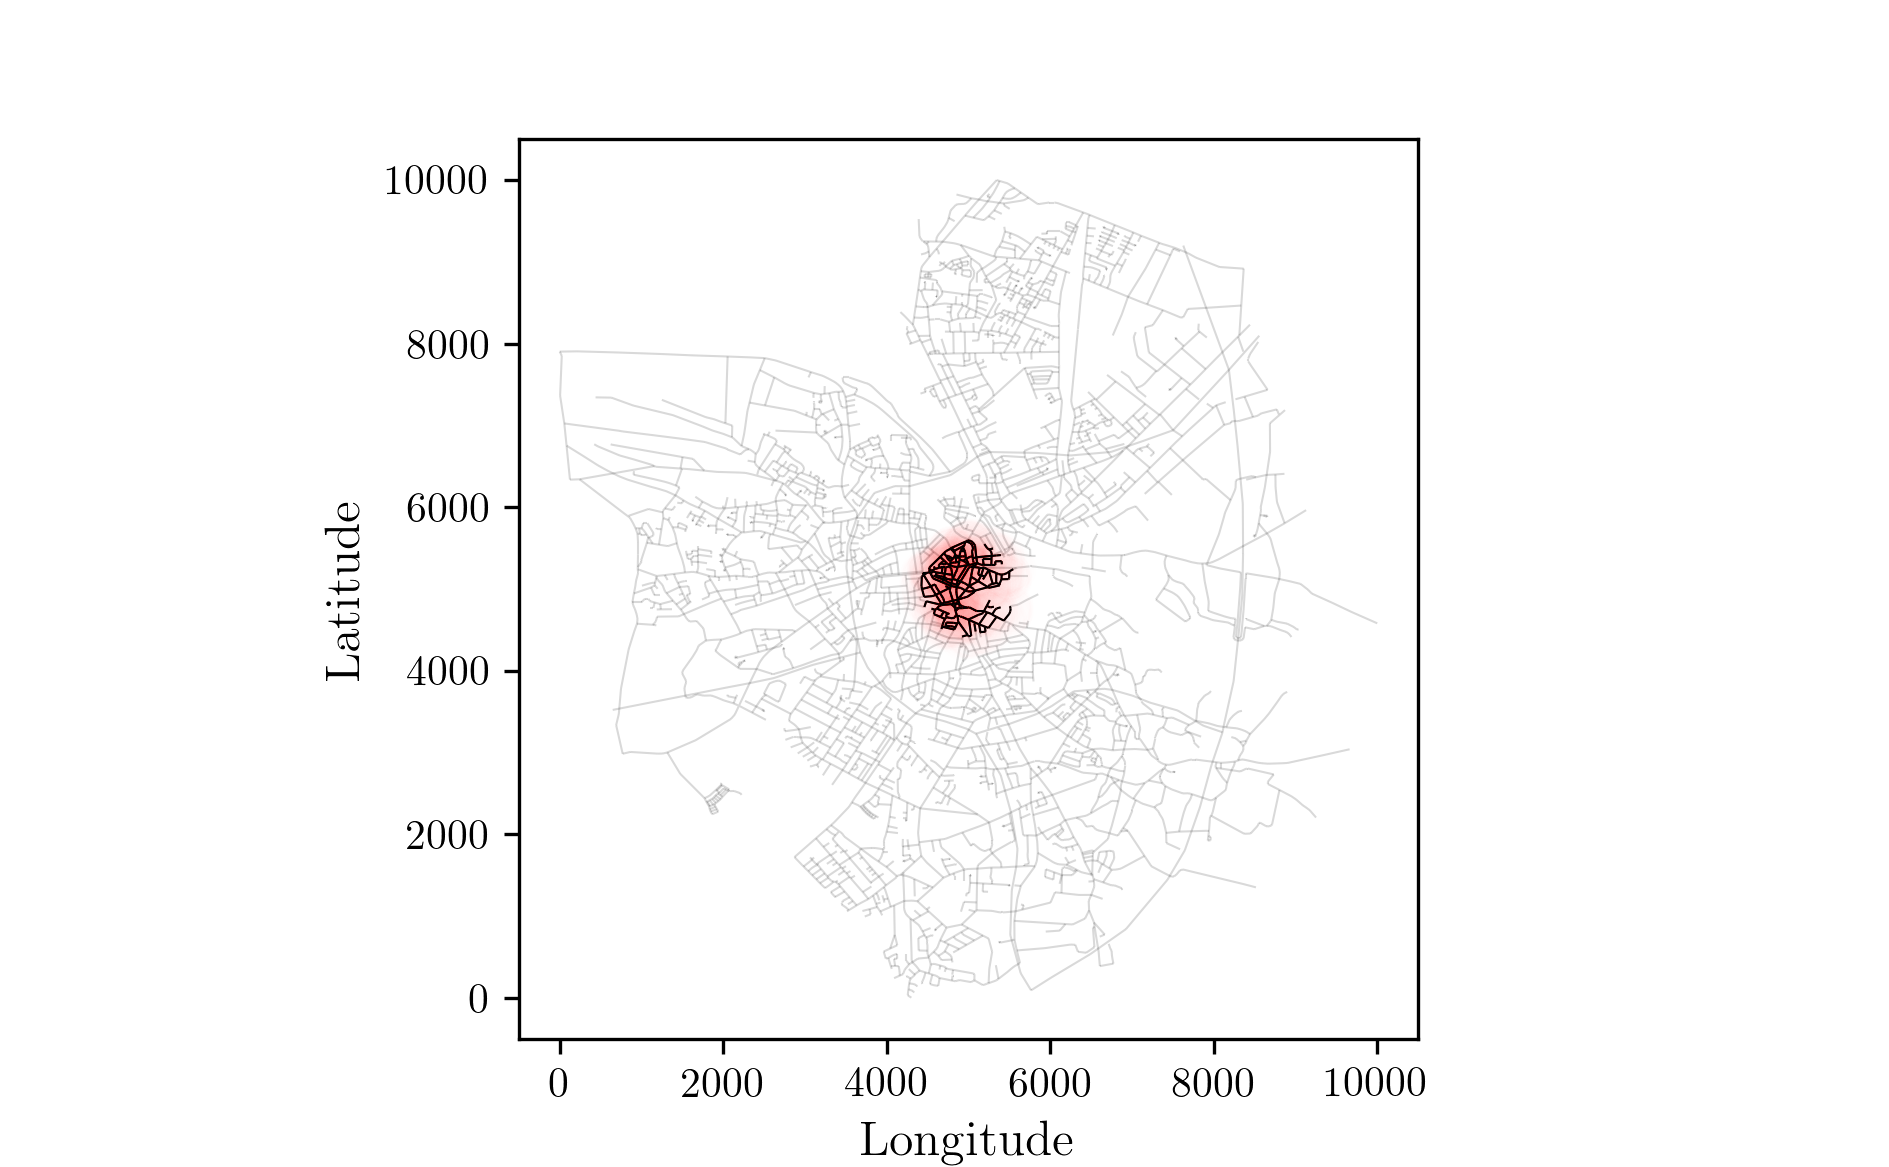
\includegraphics[scale=1]{figs/appendix-ol-small.png}
    \end{center}
    \caption[Example output of graph extractor]{An example of extracting a subsection
        of a graph. Here, I ran \texttt{./graph-extractor.py -i ../datasets/OL -x 5000 -y 5000 -d 600 --plot} to extract a subgraph of 343 vertices from the City of Oldenburg
    dataset.}
    \label{fig:appendix-ol-small}
\end{figure}

% }}}

% Download spatial datasets {{{
\section{\texttt{download-spatial-datasets.sh}}%
\label{sec:Download spatial datasets}

This script was used to download the real-world datasets prepared by
\citeauthor{graph-dataset} \cite{graph-dataset}.

\begin{verbatim}
#!/usr/bin/env bash
declare -a base_url="https://www.cs.utah.edu/~lifeifei/research/tpq"
declare -a agent='--user-agent="Mozilla/5.0 
  (Windows NT 10.0; WOW64) AppleWebKit/537.36 (KHTML, like Gecko)
  Chrome/51.0.2704.103 Safari/537.36'
declare -a files=("cal.cnode" "cal.cedge" "SF.cnode" "SF.cedge"
 "NA.cnode" "NA.cedge" "TG.cnode" "TG.cedge" "OL.cnode" "OL.cedge")

for f in "${files[@]}" ; do
    wget "$agent" "$base_url/$f" -P "../datasets/"
done
\end{verbatim}

% }}}

% evaluation.py {{{
\section{\texttt{evaluation.py}}%
\label{sec:evaluation}

This script was used to create all the plots involving timing measurement data.
There is a total of 53 lines of Python code in this script that was not written
by me, and the corresponding code has been attributed to their authors.

% }}}

\chapter{Further plots}

% Error bar
% Error bars {{{
\section{Total execution time with confidence intervals}%
\label{sec:Error bars}

In \cref{fig:main-eval-plot}, I omitted the confidence intervals on the plots
in the left column. In this section, I have plotted the same data, but with
confidence intervals included. The confidence intervals were computed by taking
the standard deviation of the total execution time samples. I have 5 samples for
each combination of $n$ (problem size) and $p$ (processing element layout size) in
\cref{fig:appendix-plot-sandy-bridge} and \cref{fig:appendix-plot-taihu-light}. For
the parallel executions in \cref{fig:appendix-plot-internet}, there are 3 samples
for each combination.

% Sandy bridge
\begin{figure}[h!]
    \begin{center}
        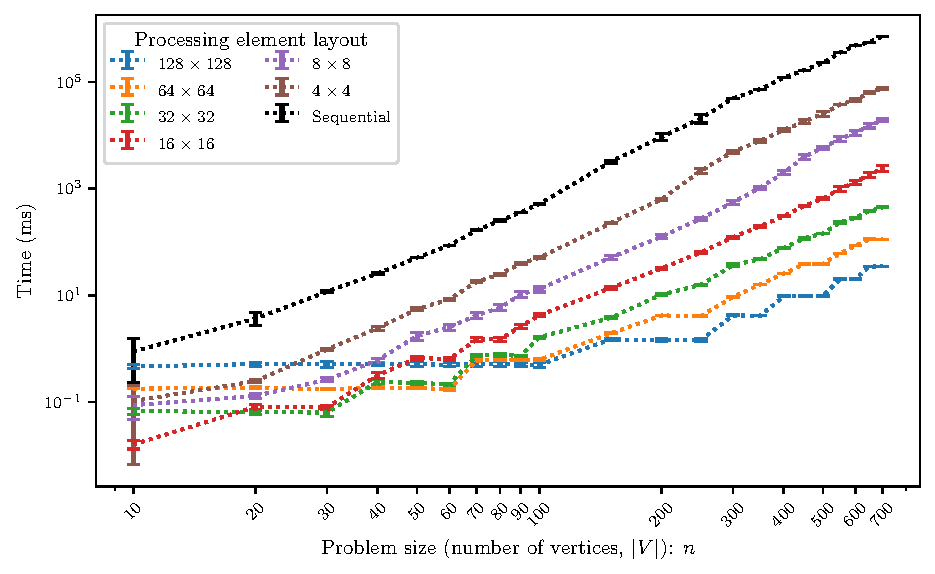
\includegraphics{figs/plots/total-time-scaling-sandy-full-width.pdf}
    \end{center}
    \caption{Multi-core processor (Sandy Bridge) total time scaling}
    \label{fig:appendix-plot-sandy-bridge}
\end{figure}

% Taihu light
\begin{figure}
    \begin{center}
        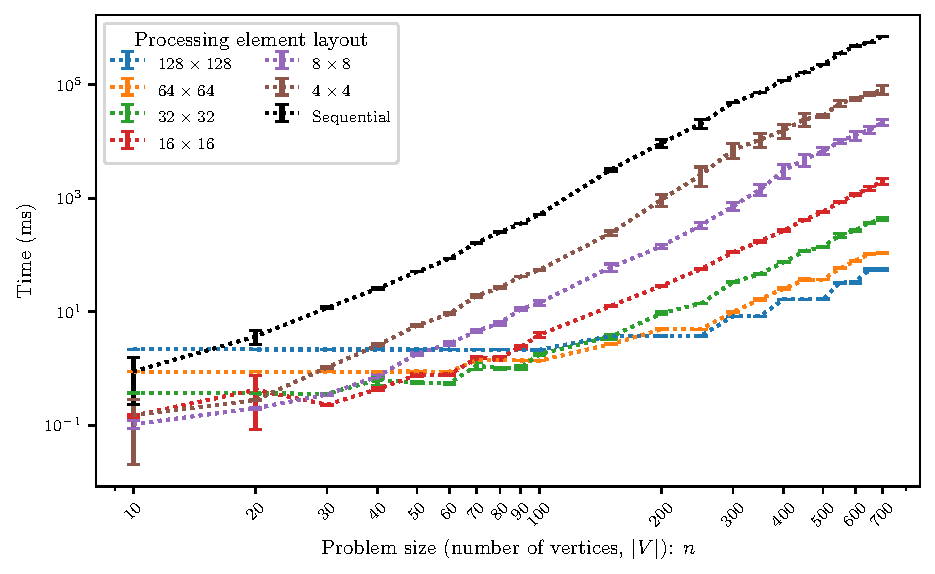
\includegraphics{figs/plots/total-time-scaling-taihu-full-width.pdf}
    \end{center}
    \caption{Supercomputer (Sunway TaihuLight) total time scaling}
    \label{fig:appendix-plot-taihu-light}
\end{figure}

% Internet
\begin{figure}
    \begin{center}
        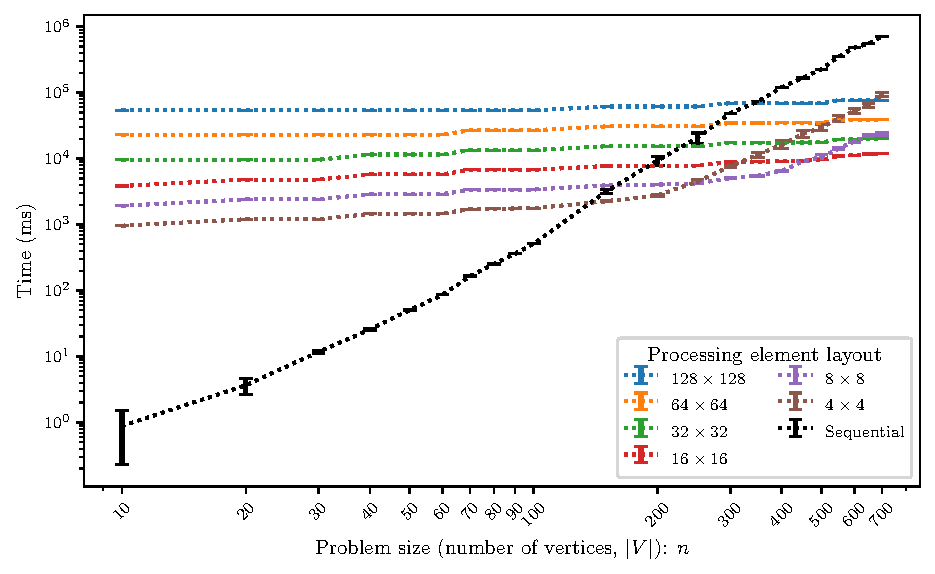
\includegraphics{figs/plots/total-time-scaling-internet-full-width.pdf}
    \end{center}
    \caption{Distributed computer (Internet) total time scaling}
    \label{fig:appendix-plot-internet}
\end{figure}

% }}}

\chapter{Algorithm examples}

% Path reconstruction
% Path reconstruction example {{{

\section{Path reconstruction}%
\label{sec:path-reconstruction}

As an example of the path reconstruction algorithm presented in
\cref{sec:APSP via repeated matrix-squaring}, consider the completed predecessor
matrix for the graph in
\cref{fig:example-graph}:
\begin{equation}
    M_{pred}=
    \begin{blockarray}{ccccccccc}
         & 0 & 1 & 2 & 3 & 4 & 5 & 6 & 7 \\
        \begin{block}{c(cccccccc)}
            0 & 0 & 5 & 0 & 0 & 1 & 2 & 2 & 7 \\
            1 & 0 & 1 & 2 & 3 & 1 & 5 & 6 & 7 \\
            2 & 0 & 5 & 2 & 3 & 1 & 2 & 2 & 7 \\
            3 & 0 & 1 & 2 & 3 & 4 & 5 & 3 & 7 \\
            4 & 0 & 1 & 2 & 3 & 4 & 5 & 6 & 7 \\
            5 & 0 & 5 & 2 & 3 & 1 & 5 & 6 & 7 \\
            6 & 0 & 1 & 2 & 3 & 4 & 5 & 6 & 7 \\
            7 & 0 & 1 & 2 & 3 & 4 & 5 & 6 & 7 \\
        \end{block}
    \end{blockarray}\;.
\end{equation}
If we want to reconstruct $0 \rightsquigarrow 1$, we start with
the list $[1]$, then prepend $M_{pred}[0,1]=5$, giving $[5,1]$. We then prepend
$M_{pred}[0,5]=2$. We continue doing this until we get $[0,2,5,1]$, where we
stop because $M_{pred}[0,0]=0$.

% }}}

\chapter{Build and test instructions}

% Building and testing
% {{{
\paragraph{Building the project}%
\label{par:Building the project}

The project uses \texttt{maven}, which can be installed with a package manager
on most unix systems. To build the code, change the working directory to \texttt{ParallelAPSP/} and run

\begin{verbatim}
mvn clean compile
\end{verbatim}

This should give the output (some lines have been omitted):

\begin{verbatim}
......
[INFO] ---------------------------------------------------------------------
[INFO] BUILD SUCCESS
[INFO] ---------------------------------------------------------------------
[INFO] Total time:  1.832 s
[INFO] Finished at: 2022-05-06T16:42:51+01:00
[INFO] ---------------------------------------------------------------------
\end{verbatim}

\paragraph{Running the unit tests}%
\label{par:Running the unit tests}

To run the unit tests, run the command

\begin{verbatim}
mvn clean test
\end{verbatim}

from the directory \texttt{ParallelAPSP/}. Note that this requires some test input
graph files to be present, otherwise some tests will fail.
The output should be (some lines have been omitted):
\begin{verbatim}
...
[INFO] Results:
[INFO] 
[INFO] Tests run: 32, Failures: 0, Errors: 0, Skipped: 0
[INFO] 
[INFO] ---------------------------------------------------------------------
[INFO] BUILD SUCCESS
[INFO] ---------------------------------------------------------------------
[INFO] Total time:  04:21 min
[INFO] Finished at: 2022-05-06T16:40:04+01:00
[INFO] ---------------------------------------------------------------------
\end{verbatim}
% }}}


% Project proposal
% {{{
\chapter{Project Proposal}

\newlength{\originalVOffset}
\newlength{\originalHOffset}
\setlength{\originalVOffset}{\voffset}   
\setlength{\originalHOffset}{\hoffset}

\setlength{\voffset}{0cm}
\setlength{\hoffset}{0cm}
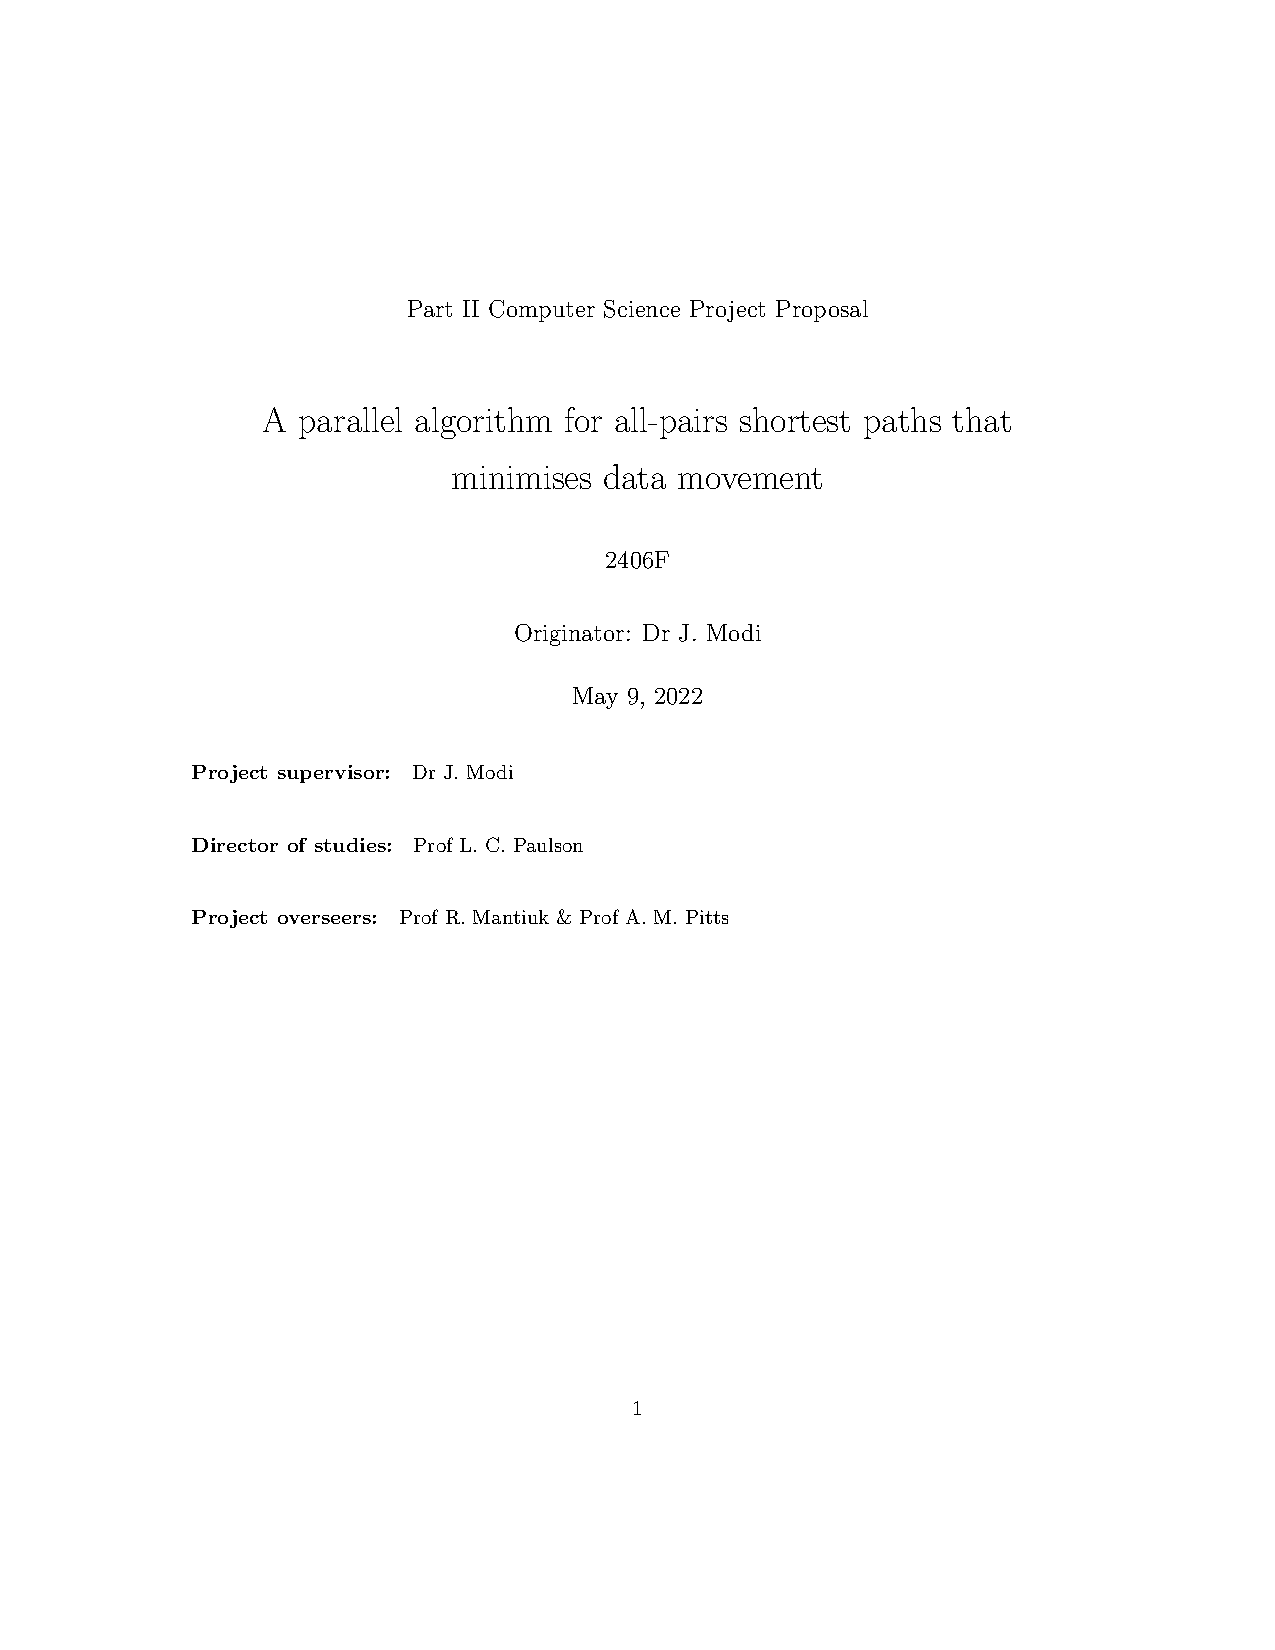
\includepdf[pages=-]{../project-proposal/build/proposal} \setlength{\voffset}{\originalVOffset}
\setlength{\hoffset}{\originalHOffset}
% }}}

% vim: foldmethod=marker
